\def\figureRandFrame{

\begin{figure}
    \centering

\scriptsize{
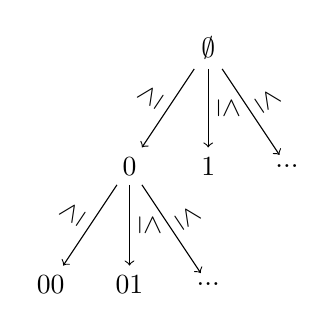
\begin{tikzpicture}
            % Root node
            \node (root) at (0,0) {$\emptyset$};
        
            % Second stage nodes
            \node (n1) at (-1,-1.5) {$0$};
            \node (n2) at (0,-1.5) {$1$};
            \node (n3) at (1,-1.5) {$...$};
        
            % Edges
            \draw[->] (root) -- (n1) node[midway, sloped, above] {$\geq$};
            \draw[->] (root) -- (n2) node[midway, sloped, above] {$\leq$};
            \draw[->] (root) -- (n3) node[midway, sloped, above] {$\leq$};
            
            % Third stage nodes
            \node (n00) at (-2,-3) {$00$};
            \node (n01) at (-1,-3) {$01$};
            \node (n02) at (0,-3) {$...$};
        
            % Edges
            \draw[->] (n1) -- (n00) node[midway, sloped, above] {$\geq$};
            \draw[->] (n1) -- (n01) node[midway, sloped, above] {$\leq$};
            \draw[->] (n1) -- (n02) node[midway, sloped, above] {$\leq$};
        
        \end{tikzpicture}
        \hspace{30pt}
        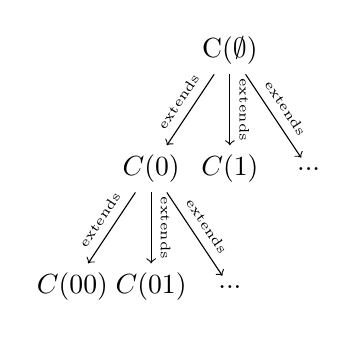
\begin{tikzpicture}
            % Root node
            \node (root) at (0,0) {C($\emptyset$)};
        
            % Second stage nodes
            \node (n1) at (-1,-1.5) {$C(0)$};
            \node (n2) at (0,-1.5) {$C(1)$};
            \node (n3) at (1,-1.5) {$...$};
        
            % Edges
            \draw[->] (root) -- (n1) node[midway, sloped, above] {\tiny{extends}};
            \draw[->] (root) -- (n2) node[midway, sloped, above] {\tiny{extends}};
            \draw[->] (root) -- (n3) node[midway, sloped, above] {\tiny{extends}};
            
            % Third stage nodes
            \node (n00) at (-2,-3) {$C(00)$};
            \node (n01) at (-1,-3) {$C(01)$};
            \node (n02) at (0,-3) {$...$};
        
            % Edges
            \draw[->] (n1) -- (n00) node[midway, sloped, above] {\tiny{extends}};
            \draw[->] (n1) -- (n01) node[midway, sloped, above] {\tiny{extends}};
            \draw[->] (n1) -- (n02) node[midway, sloped, above] {\tiny{extends}};

        \end{tikzpicture}
  

}

    \caption{R and a Kripke frame. }
    \label{fig:enter-label}
    
\end{figure}
}


\def\TableauxDevelopmentExampleFigure{
    
\begin{figure}
    \centering
    \makebox[\textwidth][c]{%
    \resizebox{0.95\textwidth}{!}{
    
    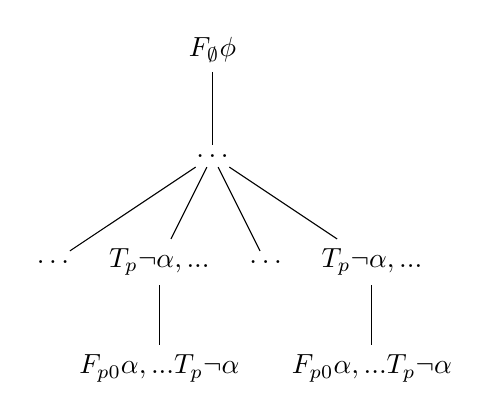
\begin{tikzpicture}[scale=0.9]
    \node {$F_{\emptyset}\phi$}
        child {node {$\ldots$}
            child {node {$\ldots$}}
            child {node {$T_{p} \neg \alpha, ...$}
                child {node {$F_{p0} \alpha, ... T_{p} \neg \alpha$}}}
            child {node {$\ldots$}}
            child {node {$T_{p} \neg \alpha, ...$}
                child {node {$F_{p0} \alpha, ... T_{p} \neg \alpha$}}}};
    \end{tikzpicture}%
    
    
    
    \hspace{0.5cm} \raisebox{1.8cm}{$\hookleftarrow$} 
    \hspace{0.5cm}
    \raisebox{1.25cm}{
    \begin{tikzpicture}[scale=0.9]
    \node {$F_{\emptyset}\phi$}
        child {node {$\ldots$}
            child {node {$\ldots$}}
            child {node {$T_{p} \neg \alpha, ...$}}
            child {node {$\ldots$}}
            child {node {$T_{p} \neg \alpha, ...$}}};
    \end{tikzpicture}
    }
    %
    }%
    }
    \caption{Example of $\hookleftarrow(T \neg \alpha ,\tau)$ and $\tau$. } 
    \label{fig:tree_expansion}
    \end{figure}
}

\def\tableauxCumulativeAndNonCumulativeExampleFigure{
    \begin{figure}
        \centering
        \scriptsize{
        \makebox[\textwidth][c]{%
        \resizebox{1\textwidth}{!}{
        \begin{tikzpicture}
            % Root node
            \node (root) at (0,0) {$F_{\emptyset} \alpha \to \neg \neg \alpha$};
            
            % Second stage nodes
            \node (n1) at (0,-1.5) {$T_{0} \alpha$};
            \draw[->] (root) -- (n1);
            
            % Third stage nodes
            \node (n2) at (0,-3) {$F_{0} \neg \neg \alpha$};
            \draw[->] (n1) -- (n2);
            
            % Fourth stage nodes
            \node (n3) at (0,-4.5) {$T_{00} \neg \alpha$};
            \draw[->] (n2) -- (n3);

            
            % Fifth stage nodes
            \node (n4) at (0,-6) {$F_{00} \alpha$};
            \draw[->] (n3) -- (n4);

            \node (n5) at (0,-7.5) {X};
            \draw[->] (n4) -- (n5);
        \end{tikzpicture}

        \hspace{1cm}

        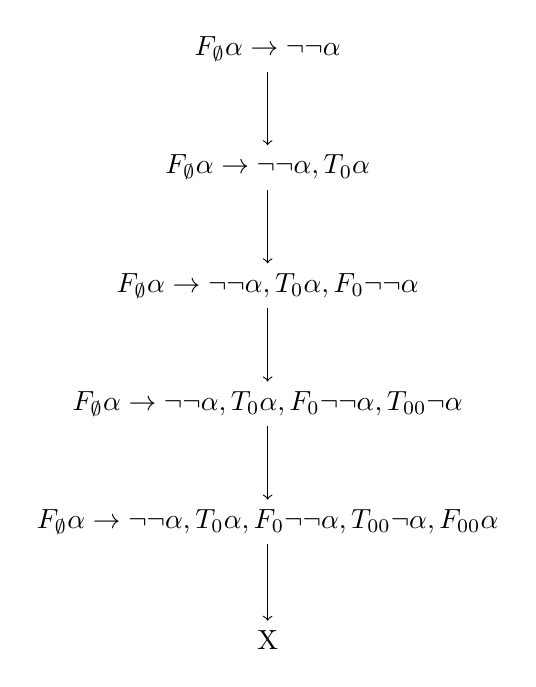
\begin{tikzpicture}
            % Root node
            \node (root) at (0,0) {$F_{\emptyset} \alpha \to \neg \neg \alpha$};
            
            % Second stage nodes
            \node (n1) at (0,-1.5) {$F_{\emptyset} \alpha \to \neg \neg \alpha, T_{0} \alpha$};
            \draw[->] (root) -- (n1);
            
            % Third stage nodes
            \node (n2) at (0,-3) {$F_{\emptyset} \alpha \to \neg \neg \alpha, T_{0} \alpha, F_{0} \neg \neg \alpha$};
            \draw[->] (n1) -- (n2);
            
            % Fourth stage nodes
            \node (n3) at (0,-4.5) {$F_{\emptyset} \alpha \to \neg \neg \alpha, T_{0} \alpha, F_{0} \neg \neg \alpha, T_{00} \neg \alpha$};
            \draw[->] (n2) -- (n3);
            
            % Fifth stage nodes
            \node (n4) at (0,-6) {$F_{\emptyset} \alpha \to \neg \neg \alpha, T_{0} \alpha, F_{0} \neg \neg \alpha, T_{00} \neg \alpha, F_{00} \alpha$};
            \draw[->] (n3) -- (n4);

            \node (n5) at (0,-7.5) {X};
            \draw[->] (n4) -- (n5);
        \end{tikzpicture}

        \hspace{1cm}

        \begin{tikzpicture}
            % Root node
            \node (root) at (0,0) {$F_{\emptyset} \alpha \to \neg \neg \alpha$};
            
            % Second stage nodes
            
            % Third stage nodes
            \node (n2) at (0,-3) {$F_{\emptyset} \alpha \to \neg \neg \alpha, T_{0} \alpha, F_{0} \neg \neg \alpha$};
            \draw[->] (root) -- (n2);
            
            % Fourth stage nodes
            \node (n3) at (0,-4.5) {$F_{\emptyset} \alpha \to \neg \neg \alpha, T_{0} \alpha, F_{0} \neg \neg \alpha, T_{00} \neg \alpha$};
            \draw[->] (n2) -- (n3);
            
            % Fifth stage nodes
            \node (n4) at (0,-6) {$F_{\emptyset} \alpha \to \neg \neg \alpha, T_{0} \alpha, F_{0} \neg \neg \alpha, T_{00} \neg \alpha, F_{00} \alpha$};
            \draw[->] (n3) -- (n4);

            \node (n5) at (0,-7.5) {X};
            \draw[->] (n4) -- (n5);
        \end{tikzpicture}
        }
        }
        }
        \caption{Example of a destructive tableaux proof tree from \cite{book1}, the intermediary structure and the non-destructive tableaux proof tree.}
        \label{fig:destructive_tableaux}
    \end{figure}
}



\def\RulesIntuitionisticSequentCalculus{


\begin{table}[h!]
    \caption{Rules for L's classical multi-consequence sequent calculus.}\label{tab:intuitionistic}
\centering
\renewcommand{\arraystretch}{3} % Adjust row height
\begin{tabular}{|c|c|}
\hline
\textbf{Rule} & \textbf{Inference} \\ \hline
Axiom  & $\AxiomC{}\UnaryInfC{$\alpha \vdash \alpha$}\DisplayProof$ \\ \hline
Weakening & $ \AxiomC{$\Gamma \vdash \Delta$}\UnaryInfC{$\Gamma, \alpha \vdash \Delta$}\DisplayProof$ \quad
$\AxiomC{$\Gamma \vdash \Delta$}\UnaryInfC{$\Gamma \vdash \Delta, \alpha$}\DisplayProof$ \\ \hline
Negation & 
$\RightLabel{\scriptsize{$\neg$R  $\neg \alpha$}}\AxiomC{$\Gamma , \vdash \alpha, \Delta$}\UnaryInfC{$\Gamma, \neg \alpha \vdash \Delta$}\DisplayProof$ \quad
$\RightLabel{\scriptsize{$\neg$L  $\neg \alpha$}}\AxiomC{$\Gamma, \alpha \vdash $}\UnaryInfC{$\Gamma \vdash \neg \alpha$}\DisplayProof$ \\ \hline
Conjunction & 
$\RightLabel{\scriptsize{$\land$L  $\alpha \land \beta$}}\AxiomC{$\Gamma, \alpha, \beta \vdash \Delta$}\UnaryInfC{$\Gamma, \alpha \land \beta \vdash \Delta$}\DisplayProof$ \quad
$\RightLabel{\scriptsize{$\land$R $\alpha \land \beta$}}\AxiomC{$\Gamma \vdash \alpha, \Delta$}\AxiomC{$\Gamma \vdash \beta, \Delta$}\BinaryInfC{$\Gamma \vdash \alpha \land \beta, \Delta$}\DisplayProof$ \\ \hline
Disjunction & 
$\RightLabel{\scriptsize{$\lor$ L  $\alpha \lor \beta$}}\AxiomC{$\Gamma, \alpha \vdash \Delta$}\AxiomC{$\Gamma, \beta \vdash \Delta$}\BinaryInfC{$\Gamma, \alpha \lor \beta \vdash \Delta$}\DisplayProof$ \quad
$\RightLabel{\scriptsize{$\lor$ R  $\alpha \lor \beta$}}\AxiomC{$\Gamma \vdash \alpha, \Delta$}\UnaryInfC{$\Gamma \vdash \alpha \lor \beta, \Delta$}\DisplayProof$ \quad
$\RightLabel{\scriptsize{$\lor$ R  $\alpha \lor \beta$}}\AxiomC{$\Gamma \vdash \beta, \Delta$}\UnaryInfC{$\Gamma \vdash \alpha \lor \beta, \Delta$}\DisplayProof$ \\ \hline
Implication & 
$\RightLabel{\scriptsize{$\to$ L  $\alpha \to \beta$}}\AxiomC{$\Gamma \vdash \alpha, \Delta$}\AxiomC{$\Gamma, \beta \vdash \Delta$}\BinaryInfC{$\Gamma, \alpha \to \beta \vdash \Delta$}\DisplayProof$ \quad
$\RightLabel{\scriptsize{$\to$ R  $\alpha \to \beta$}}\AxiomC{$\Gamma, \alpha \vdash \beta, \Delta$}\UnaryInfC{$\Gamma \vdash \alpha \to \beta, \Delta$}\DisplayProof$ \\ \hline
Quantifiers & 
$\RightLabel{\scriptsize{$\forall$ L $\forall x \alpha(x)$}}\AxiomC{$\Gamma, \alpha(t) \vdash \Delta$}\UnaryInfC{$\Gamma, \forall x \alpha(x) \vdash \Delta$}\DisplayProof$ \quad
$\RightLabel{\scriptsize{$\forall$ R $\forall x \alpha(x)$}}\AxiomC{$\Gamma \vdash \alpha(y)$}\UnaryInfC{$\Gamma \vdash \forall x \alpha(x)$}\DisplayProof$ \\ 
& 
$\RightLabel{\scriptsize{$\exists$ L $\exists x \alpha(x)$}}\AxiomC{$\Gamma, \alpha(y) \vdash \Delta$}\UnaryInfC{$\Gamma, \exists x \alpha(x) \vdash \Delta$}\DisplayProof$ \quad
$\RightLabel{\scriptsize{$\exists$ R $\exists x \alpha(x)$}}\AxiomC{$\Gamma \vdash \alpha(t), \Delta$}\UnaryInfC{$\Gamma \vdash \exists x \alpha(x), \Delta$}\DisplayProof$ \\ \hline
Contraction & 
$\AxiomC{$\Gamma, \alpha, \alpha \vdash \Delta$}\UnaryInfC{$\Gamma, \alpha \vdash \Delta$}\DisplayProof$ \quad
$\AxiomC{$\Gamma \vdash \alpha, \alpha, \Delta$}\UnaryInfC{$\Gamma \vdash \alpha, \Delta$}\DisplayProof$ \\ \hline
\end{tabular}
\end{table}
}

\def\RulesCumulativeClassicalSequentCalculus{
\begin{table}[h!]
    \caption{Cumulative Sequent Calculus Rules (Multi-Consequence).}\label{tab:cumulative}
    \centering
    \renewcommand{\arraystretch}{3}
    \begin{tabular}{|c|c|}
        \hline
        \textbf{Rule} & \textbf{Inference} \\ \hline
        Axiom & $\AxiomC{}\UnaryInfC{$\Gamma, \phi \vdash \phi, \Delta$}\DisplayProof$ \\ \hline
        
        Weakening & 
        $\AxiomC{$\Gamma \vdash \Delta$}\UnaryInfC{$\Gamma, \phi \vdash \Delta$}\DisplayProof$ \quad
        $\AxiomC{$\Gamma \vdash \Delta$}\UnaryInfC{$\Gamma \vdash \Delta, \phi$}\DisplayProof$ \\ \hline
        
        Negation & 
        $\RightLabel{\scriptsize{$\neg$R}}\AxiomC{$\Gamma , \neg \phi \vdash \phi, \Delta$}\UnaryInfC{$\Gamma, \neg \phi \vdash \Delta$}\DisplayProof$ \quad
        $\RightLabel{\scriptsize{$\neg$L}}\AxiomC{$\Gamma, \phi \vdash \Delta, \neg \phi $}\UnaryInfC{$\Gamma \vdash  \Delta, \neg \phi $}\DisplayProof$ \\ \hline
        
        Conjunction & 
        $\RightLabel{\scriptsize{$\land$L}}\AxiomC{$\Gamma, \phi, \psi, \phi \land \psi \vdash \Delta$}\UnaryInfC{$\Gamma, \phi \land \psi \vdash \Delta$}\DisplayProof$ \quad
        $\RightLabel{\scriptsize{$\land$R}}\AxiomC{$\Gamma \vdash \phi, \phi \land \psi,\Delta$}\AxiomC{$\Gamma \vdash \psi, \phi \land \psi,\Delta$}\BinaryInfC{$\Gamma \vdash \phi \land \psi, \Delta$}\DisplayProof$ \\ \hline
        
        Disjunction & 
        $\RightLabel{\scriptsize{$\lor$L}} \AxiomC{$\Gamma, \phi \lor \psi,\phi \vdash \Delta$}\AxiomC{$\Gamma, \phi \lor \psi,\psi \vdash \Delta$}\BinaryInfC{$\Gamma, \phi \lor \psi \vdash \Delta$}\DisplayProof$ \quad
        $\RightLabel{\scriptsize{$\lor$R}} \AxiomC{$\Gamma \vdash \phi \lor \psi, \psi, \Delta$}\UnaryInfC{$\Gamma \vdash \phi \lor \psi, \Delta$}\DisplayProof$ \\ \hline
        
        Implication & 
        $\RightLabel{\scriptsize{$\to$L}} \AxiomC{$\Gamma, \phi \to \psi \vdash \phi, \Delta$}\AxiomC{$\Gamma, \phi \to \psi, \psi \vdash \Delta$}\BinaryInfC{$\Gamma, \phi \to \psi \vdash \Delta$}\DisplayProof$ \quad
        $\RightLabel{\scriptsize{$\to$R}} \AxiomC{$\Gamma, \phi \vdash \psi, \phi \to \psi, \Delta$}\UnaryInfC{$\Gamma \vdash \phi \to \psi, \Delta$}\DisplayProof$ \\ \hline
        
        Quantifiers & 
        $\RightLabel{\scriptsize{$\forall$L}} \AxiomC{$\Gamma, \forall x \phi(x), \phi(t) \vdash \Delta$}\UnaryInfC{$\Gamma, \forall x \phi(x) \vdash \Delta$}\DisplayProof$ \quad
        $\RightLabel{\scriptsize{$\forall$R}} \AxiomC{$\Gamma \vdash \phi(y), \Delta$}\UnaryInfC{$\Gamma \vdash \forall x \phi(x), \Delta$}\DisplayProof$ \\
        & 
        $\RightLabel{\scriptsize{$\exists$L}} \AxiomC{$\Gamma, \phi(y) \vdash \Delta$}\UnaryInfC{$\Gamma, \exists x \phi(x) \vdash \Delta$}\DisplayProof$ \quad
        $\RightLabel{\scriptsize{$\exists$R}} \AxiomC{$\Gamma \vdash \phi(t), \Delta$}\UnaryInfC{$\Gamma \vdash \exists x \phi(x), \Delta$}\DisplayProof$ \\ \hline
    \end{tabular}
\end{table}
}




\def\RulesClassicalSequentCalculus{

\begin{table}[h!]
    \caption{Rules for L's classical multi-consequence sequent calculus.}\label{tab:classical}
\centering
\renewcommand{\arraystretch}{3} % Adjust row height
\begin{tabular}{|c|c|}
\hline
\textbf{Rule} & \textbf{Inference} \\ \hline
Axiom  & $\AxiomC{}\UnaryInfC{$\alpha \vdash \alpha$}\DisplayProof$ \\ \hline
Weakening & $ \AxiomC{$\Gamma \vdash \Delta$}\UnaryInfC{$\Gamma, \alpha \vdash \Delta$}\DisplayProof$ \quad
$\AxiomC{$\Gamma \vdash \Delta$}\UnaryInfC{$\Gamma \vdash \Delta, \alpha$}\DisplayProof$ \\ \hline
Negation & 
$\RightLabel{\scriptsize{$\neg$R  $\neg \alpha$}}\AxiomC{$\Gamma , \vdash \alpha, \Delta$}\UnaryInfC{$\Gamma, \neg \alpha \vdash \Delta$}\DisplayProof$ \quad
$\RightLabel{\scriptsize{$\neg$L  $\neg \alpha$}}\AxiomC{$\Gamma, \alpha \vdash \Delta$}\UnaryInfC{$\Gamma \vdash \neg \alpha, \Delta$}\DisplayProof$ \\ \hline
Conjunction & 
$\RightLabel{\scriptsize{$\land$L  $\alpha \land \beta$}}\AxiomC{$\Gamma, \alpha, \beta \vdash \Delta$}\UnaryInfC{$\Gamma, \alpha \land \beta \vdash \Delta$}\DisplayProof$ \quad
$\RightLabel{\scriptsize{$\land$R $\alpha \land \beta$}}\AxiomC{$\Gamma \vdash \alpha, \Delta$}\AxiomC{$\Gamma \vdash \beta, \Delta$}\BinaryInfC{$\Gamma \vdash \alpha \land \beta, \Delta$}\DisplayProof$ \\ \hline
Disjunction & 
$\RightLabel{\scriptsize{$\lor$ L  $\alpha \lor \beta$}}\AxiomC{$\Gamma, \alpha \vdash \Delta$}\AxiomC{$\Gamma, \beta \vdash \Delta$}\BinaryInfC{$\Gamma, \alpha \lor \beta \vdash \Delta$}\DisplayProof$ \quad
$\RightLabel{\scriptsize{$\lor$ R  $\alpha \lor \beta$}}\AxiomC{$\Gamma \vdash \alpha, \Delta$}\UnaryInfC{$\Gamma \vdash \alpha \lor \beta, \Delta$}\DisplayProof$ \quad
$\RightLabel{\scriptsize{$\lor$ R  $\alpha \lor \beta$}}\AxiomC{$\Gamma \vdash \beta, \Delta$}\UnaryInfC{$\Gamma \vdash \alpha \lor \beta, \Delta$}\DisplayProof$ \\ \hline
Implication & 
$\RightLabel{\scriptsize{$\to$ L  $\alpha \to \beta$}}\AxiomC{$\Gamma \vdash \alpha, \Delta$}\AxiomC{$\Gamma, \beta \vdash \Delta$}\BinaryInfC{$\Gamma, \alpha \to \beta \vdash \Delta$}\DisplayProof$ \quad
$\RightLabel{\scriptsize{$\to$ R  $\alpha \to \beta$}}\AxiomC{$\Gamma, \alpha \vdash \beta, \Delta$}\UnaryInfC{$\Gamma \vdash \alpha \to \beta, \Delta$}\DisplayProof$ \\ \hline
Quantifiers & 
$\RightLabel{\scriptsize{$\forall$ L $\forall x \alpha(x)$}}\AxiomC{$\Gamma, \alpha(t) \vdash \Delta$}\UnaryInfC{$\Gamma, \forall x \alpha(x) \vdash \Delta$}\DisplayProof$ \quad
$\RightLabel{\scriptsize{$\forall$ R $\forall x \alpha(x)$}}\AxiomC{$\Gamma \vdash \alpha(y), \Delta$}\UnaryInfC{$\Gamma \vdash \forall x \alpha(x), \Delta$}\DisplayProof$ \\ 
& 
$\RightLabel{\scriptsize{$\exists$ L $\exists x \alpha(x)$}}\AxiomC{$\Gamma, \alpha(y) \vdash \Delta$}\UnaryInfC{$\Gamma, \exists x \alpha(x) \vdash \Delta$}\DisplayProof$ \quad
$\RightLabel{\scriptsize{$\exists$ R $\exists x \alpha(x)$}}\AxiomC{$\Gamma \vdash \alpha(t), \Delta$}\UnaryInfC{$\Gamma \vdash \exists x \alpha(x), \Delta$}\DisplayProof$ \\ \hline
Contraction & 
$\AxiomC{$\Gamma, \alpha, \alpha \vdash \Delta$}\UnaryInfC{$\Gamma, \alpha \vdash \Delta$}\DisplayProof$ \quad
$\AxiomC{$\Gamma \vdash \alpha, \alpha, \Delta$}\UnaryInfC{$\Gamma \vdash \alpha, \Delta$}\DisplayProof$ \\ \hline
\end{tabular}
\end{table}
}
